\chapter{Basics}

\section{A first example}

Let's start with an easy example. Assume we want to define a function which can add two integers:

\ceditor{add.c}{code/basics/add_simple.c}

If we want to prove, that this function is correct, we can define a \emph{function contract}, which specifies the behaviour we expect:

\ceditor{add.c}{code/basics/add_c1.c}

As you can see, function contracts are written as a special comment section  (\mintinline{c}{/*@ ... */}) just above the function signature. The \emph{ensures} keyword introduces a \emph{postcondition}, i.e. a formula which must be true when the function returns. ACSL offers the keyword \textbf{\textbackslash result} as a placeholder for the return value of a function. 

We can try proving this contract by invoking Frama-C on our C file:

\SU{user=user,host=linux,color=lime}
\begin{ubuntu}
frama-c-gui add.c
\end{ubuntu}

This will start the graphical user interface of Frama-C:

\begin{center}
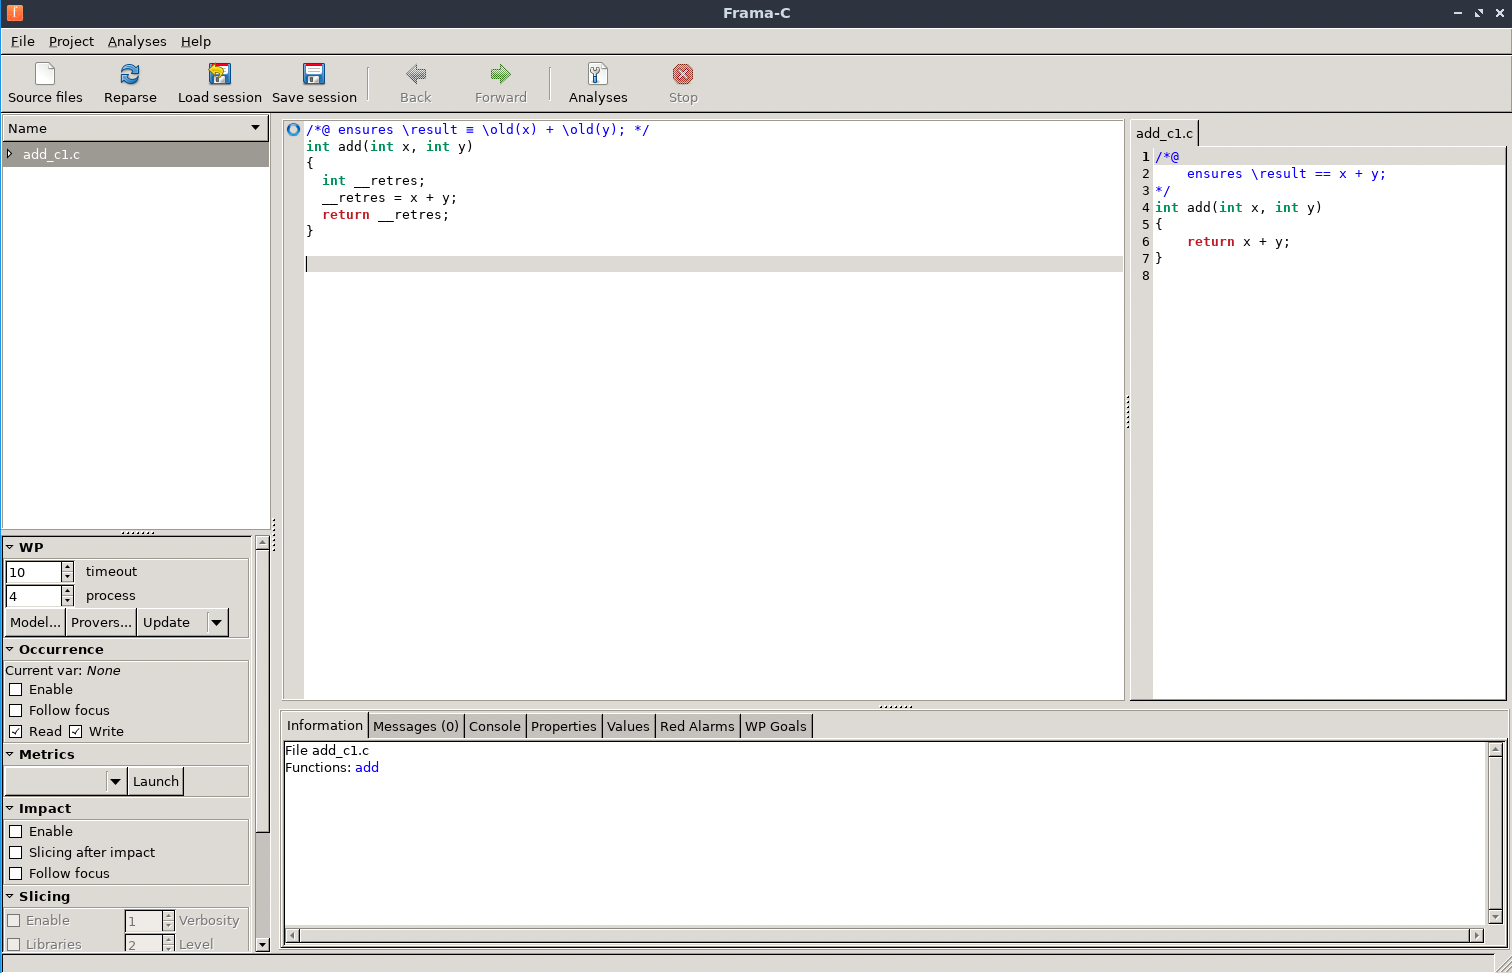
\includegraphics[width=\textwidth]{images/frama_c_add_c1.png}
\end{center}

There are a few important parts in the Frama-C GUI. On the left side we have an overview of open files and functions defined therein. On the right side we can see our original function and our contract. In between we can see the output of the parser of Frama-C, for the most part we can just accept it as a sightly altered version of the code we provided, which has exactly the same meaning as the one we wrote. 

If you look carefully, the function contract has been slightly pretty printed in the parsed view (e.g. the $==$ has been changed to $\equiv$). This will happen with many of the mathematical definitions we are going to use later on as well. 

Probably the most interesting part for us is the little blue circle next to our contract in the middle window. This indicates, that we have not yet proven the contract. So let's start with that. 

When we want to prove function contracts we can do so in multiple ways. In the middle window right-click on the function name (i.e. \textbf{add}) and select "Prove function annotations by WP". This will turn the blue circle into a green bullet, which indicates that Frama-C was successful in proving our contract. 

The careful reader might object at this point, and say something intelligent along the lines of "but what about overflows?". And indeed, those might very well happen if we add up two integers that are big enough. When Frama-C proved our contract it did so under the assumption that no runtime error occured. However, as mere mortal programmers, we do have to take into account the finite machine precision of our hardware. 

Luckily, Frama-C can help us with that. It provides a plugin called WP-RTE (Run Time Errors), which can automatically insert assertions into our code to check for runtime errors, such as overflows. To do so, we right-click on our function name again and select "Insert wp-rte guards". If you don't see this option, then the RTE plugin has not been activated yet. In that case, click on "Analyses" in the header menu (the one that looks like a sheet of paper and a tool in front of it). Then select "WP" in the list on the left, unfold "Computational Strategies" and select "-wp-rte". 

Now we can try and prove our function annotations again. You will see, that our own contract still turns green, however, the automatically inserted RTE guards are yellow, which means that Frama-C could not prove those for all possible inputs to our function. 

\section{Preconditions}

To allow Frama-C to prove the absence of runtime errors, we have to give certain guarantees that are valid when we call our \textbf{add} function. These guarantees are called \emph{preconditions}. Pre- and postconditions are the bread and butter of functional contracts. We could formulate the process of what Frama-C is doing as the following: If we can guarantee, that all preconditions are valid when we call our function, and the function itself terminates, then Frama-C will prove that the given postcondition(s) are also satisfied. 

In our case we can state the following:

\ceditor{add.c}{code/basics/add_pre.c}

Precoditions are introduced by the \emph{requires} keywoard. As you can see, ACSL allows for a nicer syntax when it comes to defining conditionals, as we can define the lower and upper limit of $x+y$ in one formula instead of two (i.e. \mintinline[breaklines]{c}{INT_MIN <= (x + y) && (x + y) <= INT_MAX}). 

You cannot edit your code in Frama-C directly, so you have to do your changes in a separate editor and then reparse the file. You can also just close the current Frama-C window, change the source code and then open it again. We can tell Frama-C to immediately insert the RTE guards and perform the contract analysis:

\begin{ubuntu}
frama-c-gui -wp -wp-rte add.c
\end{ubuntu}

If we check the status of our function annotations, all of them should be green now. The only blue circle that remains is our precondition, since that can of course not be proven without actually calling the function. 

\section{Partial vs complete specification}

At this point we might assume that we were successful in specifying the behaviour and proving the correctness of our implementation of the \textbf{add} function. Unfortunately we are not finished yet. To see that, let us observe what happens if we actually try and call our \textbf{add} function from another function:

\ceditor{add.c}{code/basics/add_main.c}

As you can see, we can also write ACSL annotations with single line comments. The \emph{assert} keyword allows us to insert assertions about our program variables at any point in our code. Here we also included a global variable v, which after calling \textbf{add} should still have the same value it had before. When we try and run

\begin{ubuntu}
frama-c-gui -wp -wp-rte add.c
\end{ubuntu}

now, we will get the following for the main function:

\begin{center}
    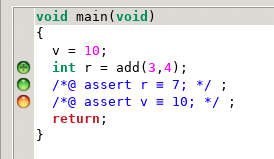
\includegraphics[width=0.5\textwidth]{images/frama_c_add_main.png}
\end{center}

The green bullet next to the \textbf{add} function tells us that we are fulfilling the preconditions of the \textbf{add} function, and the green bullet on the next line shows that the return value is indeed 7. However, Frama-C failed to prove that the global variable v has not changed value. 

This is due to the fact, that we have not specified anything about the memory locations that our \textbf{add} function is allowed to alter. Therefore, Frama-C cannot simply assume that no global variables have been changed once we call \textbf{add}. We have to list all the locations that \textbf{add} can read/write to in the contract of our function, which we can do by using the assigns keyword. With that in place, our file looks as follows:

\ceditor{add.c}{code/basics/add.c}

ACSL provides the special value \textbf{\textbackslash nothing} to express that the function is not changing any global state. If we run the same command as before, we will now see that also the second assert statement turns green: 

\begin{center}
    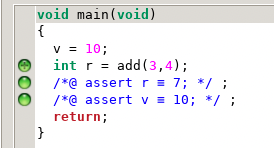
\includegraphics[width=0.5\textwidth]{images/frama_c_add_all_green.png}
\end{center}

This illustrates an important fact about using contracts for function specification. It is sometimes very difficult to find a complete specification (that is one that covers every aspect of the behaviour we are expecting). Sometimes, if for example we know all the calling contexts of the function we are trying to specify, it is enough to just use a partial specification. If a certain contract actually fully specifies an implementation is outside of the scope of what ACSL can do, for that we have to evaluate against a more abstract model of our software system.

So far we have only dealt with contracts that had one pre- and one postcondition. We can however specify arbitrarily many by either having multiple requires/ensures clauses, or using the logical operators \mintinline{c}{&&} and \mintinline{c}{||} respectively. We will make use of that in the next chapter, and you might need it in the exercises. 

\section{Exercises}

\subsection{Abs function}

Implement the \textbf{abs} function, which shall return the absolute value of the integer parameter x given to it:

\ceditor{abs.c}{exercises/basics/abs.c}

Write the necessary specification for the \textbf{abs} function and prove its correctness. For specifying the postcondition, you may want to use the \mintinline{c}{==>} (implies) operator. For further details consult \cite{baudin_acsl_nodate}. 

\subsection{Max function}

Implement the \textbf{max} function, which shall return the bigger of the two input parameters:

\ceditor{max.c}{exercises/basics/max.c}

This time, write your own main function and try to include and prove some assertions! 

\subsection{Alphanumeric function}

Have a look at the following function:

\ceditor{alphanumeric.c}{exercises/basics/alphanumeric.c}

The \textbf{is\textunderscore alphanumeric} function takes a character as input and shall return 1 if it is a letter (either lower or upper case) or a digit (i.e. '0' - '9'). 

\subsection{Days per month}

Assume we have the following given function, which given a month (i.e. an integer between 1 and 12) returns the number of days in that month:

\ceditor{number\textunderscore of\textunderscore days.c}{exercises/basics/number_of_days.c}

Write the required pre- and postconditions for this function. You will realize, that the postcondition is quite awkward to write, luckily ACSL can help us here. ACSL provides the \textbf{\textbackslash in} keyword, that allows to reason about sets like this: \mintinline{c}{//@ assert 3 \in {1, 2, 3, 4};}. Try using it in your postcondition! 
